\lstset{style=pythoninlinestyle}

\section{РЕКОМЕНДАЦИИ ПО ПРАКТИЧЕСКОМУ ИСПОЛЬЗОВАНИЮ ПРОГРАММНОГО СРЕДСТВА}
\label{sec:manual}

\subsection{Разработка инструкции (руководства) пользователя}
\label{sub:manual:1}

Поскольку программное средство написано н аязыке Python 3, для его работы требуется интерпретатор python версии 3.0 и выше. Перед началом работы  требуется активировать виртуальное окружение venv, которое установит необходимые переменные окружения путем вызова \lstinline!source ./venv/bin/activate! в оболочке командной строки bash, zshell, или аналогичной.

\subsubsection{Симуляция}

Запуск симуляции эксперимента происходит через файл fuzzysim.py в корневой директории приложения. В общем виде команда запуска симуляции выглядит как:

\begin{lstlisting}[style=pythonstyle,caption={  }, label=lst:func:1]
  fuzzysim.py [-h] [-w WAY_CONFIG_FILE] [-l LATENCY]                   [-c BRAKE_CONTROLLER] [-n] [-s] distance speed
\end{lstlisting}

Ключи командной строки обозначают следующее:

\begin{itemize}
	\item \lstinline! -h!: отобразить справку по командам;
	\item \lstinline! -w!: файл с конфигурацией симулируемого пут;
	\item \lstinline! -l!: значение задержки в системе управления в секундах, число с плавающей запятой;
	\item \lstinline! -c!: имя модуля нечеткого контроллера. Файл с исходным кодом контроллера должен быть расположен в папке \lstinline!brake_controller!;
	\item \lstinline! -n!: не отображать графики с результатами эксперимента;
	\item \lstinline! -s!: вместо конечных результатов эксперимента вывести собранную телеметрию в формате Comma Separated Values (CSV);
	\item \lstinline! distance!: S0, начальное расстояние до препятствия, в метрах;
	\item \lstinline! speed!: V0, начальная скорость платформы.
\end{itemize}

Вывод в формате CSV можно сохранить в файл путем перенаправления потока ввода. Вывод нескольких экспериментов можно объединять в один файл для последующего сравнения.

Вывод результата эксперимента показывает:

\begin{itemize}
	\item \lstinline! T!: модельное время завершения эксперимента;
	\item \lstinline! S!: расстояние до препятствия на момент окончания симуляции;
	\item \lstinline! V!: скорость платформы на момент окончания симуляции;
	\item \lstinline! A!: скорость платформы на момент окончания симуляции;
	\item \lstinline! Simulation time!: общее машинное время симуляции.
\end{itemize}

На рис. 4.1 и 4.2 представлены результаты удачного (платформа остановилась успешно) и неудачного (платформа столкнулась с препятствием) экспериментов соответственно.

\begin{figure}[ht]
  \centering
  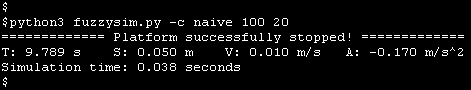
\includegraphics[scale=0.8]{4-1.png}
  \caption{Результат удачного эксперимента }
  % \label{fig:func:1}
\end{figure}

\begin{figure}[ht]
  \centering
  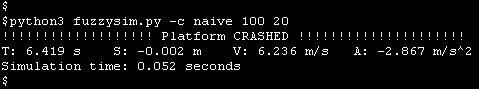
\includegraphics[scale=0.8]{4-2.png}
  \caption{Результат неудачного эксперимента }
  % \label{fig:func:1}
\end{figure}

После окончания эксперимента выводятся графики результатов:


\begin{itemize}
	\item график зависимости расстояния до препятствия от времени, по оси абсцисс время в секундах, по оси ординат расстояние до препятствия в метрах;
	\item график зависимости скорости от времени, по оси абсцисс время в секундах, по оси ординат скорость платформы в метрах в секунду;
	\item график зависимости ускорения от времени, по оси абсцисс время в секундах, по оси ординат ускорение в метрах в секунду за секунду;
	\item график зависимости рывка от времени, по оси абсцисс время в секундах, по оси ординат рывок в метрах в секунду за секунду за секунду.
\end{itemize}


Графики выводятся с помощью пакета matplotlib, который позволяет проводить с графиками различные манипуляции:

\begin{itemize}
	\item отображать точные значения по оси абсцисс и ординат под указателем мыши;
	\item изменять масштаб;
	\item перемещать график в окне просмотра;
	\item настраивать размеры полей графика;
	\item сохранять график в виде графического файла;
	\item перемещаться по истории изменений графика назад;
	\item перемещаться по истории изменений графика вперед;
	\item восстанавливать исходных вид графика.
\end{itemize}


Графики выводятся в разных окнах, что позволяет располагать их рядом для одновременного просмотра. На рисунке 4.3 приведен скриншот графика скорости.

\begin{figure}[ht]
  \centering
  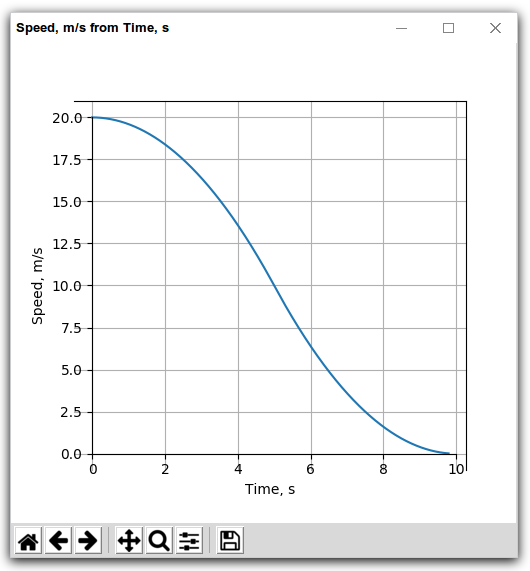
\includegraphics[scale=0.5]{4-3.png}
  \caption{График зависимости скорости от времени }
  % \label{fig:func:1}
\end{figure}


\subsubsection{ Отображение сохраненных результатов эксперимента }

Отображение сохраненных результатов эксперимента запускается через файл \lstinline!plot.py! в корневой директории приложения. Этот файл является точчкой входа модуля визуализации телеметрии. В общем виде команда запуска симуляции выглядит как:


\begin{lstlisting}[style=pythonstyle,caption={  }, label=lst:func:1]
  plot.py [-h] csv_file
\end{lstlisting}

Ключи командной строки обозначают следующее:

\begin{itemize}
	\item \lstinline! -h!: отобразить справку по командам;
	\item \lstinline! csv_file!: файл с сохраненными результатами экспериментов в формате CSV.
\end{itemize}

В результате выполнения этой команды будут выведены графики результатов, описанные в п. 4.1.1.

В случае, если в файле сохранено несколько экспериментов, одинаковые (отображающие одни и те же зависимости) графики разных экспериментов будут наложены друг на друга и отмечены в легенде по номерам, начиная с  нуля. При этом графики разных экспериментов выводятся разными цветами, причем соответствие цветов номеру эксперимента сохраняется на разных графиках, например, если нулевой эксперимент на графике скорости отображен синим цветом, то и на графике расстояния он будет отображен синим цветом.

На рис. 4.4 приведен пример графика скорости трех экспериментов.

\begin{figure}[ht]
  \centering
  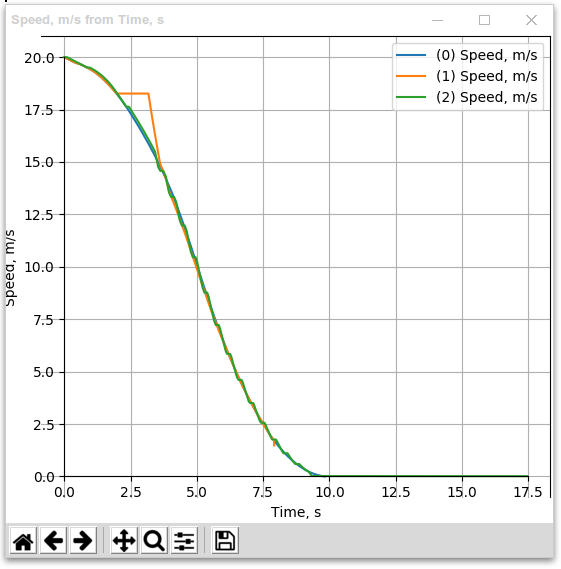
\includegraphics[scale=0.5]{4-4.png}
  \caption{График зависимости скорости от времени }
  % \label{fig:func:1}
\end{figure}

\subsubsection{ Генерация правил нечеткого контроллера }

Генерация правил нечеткого контроллера запускается через \lstinline!generate.py! в корневой директории приложения. В общем виде команда запуска симуляции выглядит как:

\begin{lstlisting}[style=pythonstyle,caption={  }, label=lst:func:1]
  generate.py [-h] [-i] csv_file terms
\end{lstlisting}

Ключи командной строки обозначают следующее:

\begin{itemize}
	\item \lstinline! -h!: отобразить справку по командам;
	\item \lstinline! -i!: генерировать интервальные функции принадлежностей для выходных переменных;
	\item \lstinline! csv_file!: файл с сохраненными результатами экспериментов в формате CSV, которые будут приняты за эталон;
	\item \lstinline! terms!: количество термов, на которые необходимо разбить области определения переменных;
\end{itemize}

Сгенерированный конфигурационный файл с правилами и лингвистическими переменными будет выведен в стандартный вывод. Его можно сохранить в файл используя перенаправление потоков.

\subsection{ Разработка инструкции (руководства) программиста }

Разрабатываемое программное средство предоставляет очень простой API для разработчиков алгоритмов нечетких контроллеров.

В качестве примера можно рассмотреть <<наивный>> контроллер. он представляет собой python-модуль, размещенный в папке \lstinline!brake_controller!. Модуль должен предоставлять функцию\lstinline! get_a(current_s, current_v, current_a)!. Функция должна возвращать число с плавающей запятой, ускорение в метрах в секунду за секунду, в текущем кванте модельного времени, соответствующее текущим расстоянию до препятствия, скорости и ускорению. Входные аргументы:

\begin{itemize}
	\item \lstinline! current_s!: текущая расстояние до препятствия, в метрах;
	\item \lstinline! current_v!: текущая скорость, в метрах в секунду;
	\item \lstinline! current_a!: текущее ускорение, в метрах в секунду за секунду.

\end{itemize}

Код <<наивного контроллера>>, приведенные для примера:

\begin{lstlisting}[style=pythonstyle,caption={  }, label=lst:func:1]
import math
applying_a = 0
time_quantum = 0.001
search_j = None
current_j = None
const_a = None
def get_a(current_s, current_v, current_a):
  global applying_a, search_j, current_j, const_a
  if search_j is None:
     const_a = -current_v ** 2 / (2 * current_s)
     time_a_const = 2 * current_s / current_v
     search_j=abs((const_a-current_a)*2/(time_a_const / 2))
     current_j = -search_j
  if current_j == -search_j:
     current_j=math.copysign(search_j,const_a*2- applying_a)
  applying_a += current_j * time_quantum
  return applying_a
\end{lstlisting}
